\documentclass[12pt,a4paper]{article}
\usepackage[utf8]{vietnam}
\usepackage{amsmath,amssymb}
\usepackage{tabularx}
\usepackage{tikz}
\usetikzlibrary{calc,angles,quotes,arrows.meta,patterns}
\usepackage{xcolor}
\usepackage{enumitem}
\usepackage{fancyhdr}
\usepackage{graphicx}
\usepackage[top=0.9cm, bottom=0.9cm, left=1.2cm, right=1.2cm]{geometry}
\usepackage[dethi]{ex_test}
\SAOPTN{widthSA=3.2,heightSA=0.62}

\setlength{\headheight}{15pt}
\setlength{\parskip}{0pt}

\pagestyle{fancy}
\fancyhf{}
\rhead{\textit{Môn Toán 9 -- Đề số 10}}
\lhead{\textit{Bộ đề ôn tập Giữa học kì I}}
\cfoot{\thepage}

\begin{document}

% --- KHUNG TIÊU ĐỀ ĐỀ THI ---
\noindent
\begin{tabularx}{\linewidth}{X r}
\textbf{TRƯỜNG THCS: \dotfill} & \textbf{ĐỀ KIỂM TRA ĐỊNH KỲ GIỮA HỌC KỲ I} \\
\textbf{Họ và tên: \dotfill} & \textbf{NĂM HỌC 2026 -- 2027} \\
\textbf{Lớp: \dotfill \quad SBD: \dotfill} & \textbf{Môn: TOÁN 9} \\
\hline
\end{tabularx}
\vspace{2mm}

\begin{center}
  \textbf{\large ĐỀ ÔN TẬP GIỮA HỌC KỲ I -- ĐỀ SỐ 10}\\
  \textit{Thời gian làm bài: 90 phút (Không kể thời gian phát đề)}
\end{center}
\vspace{1mm}

% --- PHẦN I ---
\noindent\textbf{\large PHẦN I. CÂU TRẮC NGHIỆM NHIỀU PHƯƠNG ÁN LỰA CHỌN (3,0 điểm)}

\textit{Thí sinh trả lời từ câu 1 đến câu 12. Mỗi câu hỏi thí sinh chỉ chọn một phương án duy nhất.}

\vspace{1mm}
\begin{ex}
Số nghiệm của phương trình $\left(x + \frac{1}{3}\right)(x - 3) = 0$ là:
\choice
{1}
{3}
{\True 2}
{Vô nghiệm}
\end{ex}

\begin{ex}
Bất phương trình $4x > 3x + 7$ có nghiệm là:
\choice
{$x > -7$}
{$x \le -7$}
{\True $x > 7$}
{$x < -7$}
\end{ex}

\begin{ex}
Nghiệm của hệ phương trình $\begin{cases} x + y = 7 \\ x - y = -1 \end{cases}$ là:
\choice
{$(x; y) = (4; 3)$}
{$(x; y) = (5; 4)$}
{$(x; y) = (-3; 4)$}
{\True $(x; y) = (3; 4)$}
\end{ex}

\begin{ex}
Nếu $a, b, c$ là ba số mà $a < b$ và $ac > bc$ thì $c$ là:
\choice
{Số 0}
{Số dương}
{\True Số âm}
{Số tùy ý}
\end{ex}

\begin{ex}
Bất phương trình nào dưới đây là bất phương trình bậc nhất một ẩn?
\choice
{$\frac{1}{x} - 1 > 0$}
{$x^2 > 0$}
{\True $\frac{1}{3}x + 2 < 0$}
{$0 \cdot x + 3 > 0$}
\end{ex}

\begin{ex}
Những số nào sau đây là nghiệm của bất phương trình $2x - 10 < 0$?
\choice
{\True $-2; 0$}
{$0; 5$}
{$-2; 0; 5$}
{$-2; 4; 6$}
\end{ex}

\begin{ex}
Cho tam giác $ABC$ vuông tại $A$, đường cao $AH$. Trong tam giác vuông $ABH$, $\cos B$ bằng:
\begin{center}
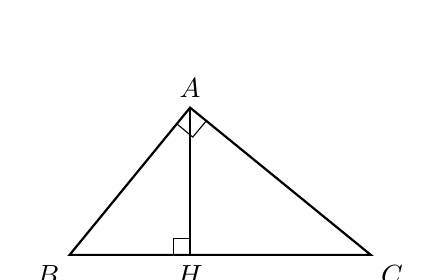
\begin{tikzpicture}[scale=0.85]
  \coordinate (B) at (0,0);
  \coordinate (H) at (1.8,0);
  \coordinate (C) at (4.5,0);
  \coordinate (A) at (1.8,2.2);
  \draw[thick] (B) node[below left]{$B$} -- (C) node[below right]{$C$} -- (A) node[above]{$A$} -- cycle;
  \draw[thick] (A) -- (H) node[below]{$H$};
  \draw (A) ++(-0.2,-0.24) -- ++(0.24,-0.2) -- ++(0.2,0.24);
  \draw (H) ++(0,0.25) -- ++(-0.25,0) -- ++(0,-0.25);
\end{tikzpicture}
\end{center}
\choice
{\True $\frac{BH}{AB}$}
{$\frac{AH}{AB}$}
{$\frac{BH}{AH}$}
{$\frac{AB}{AC}$}
\end{ex}

\begin{ex}
Cho tam giác $ABC$ vuông tại $A$, $AB = 4$ và $BC = 5$. Khẳng định nào sau đây là đúng?
\choice
{$\sin B = \frac{4}{5}$}
{$\cos B = \frac{3}{5}$}
{\True $\tan B = \frac{3}{4}$}
{$\cot B = \frac{3}{4}$}
\end{ex}

\begin{ex}
Cho đường tròn $(O)$ và hai điểm $A, B$ nằm trên đường tròn. Góc ở tâm của đường tròn $(O)$ là:
\begin{center}
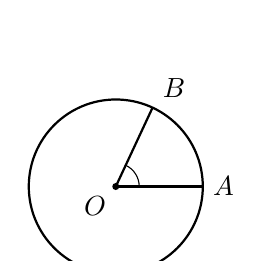
\begin{tikzpicture}[scale=0.85]
  \coordinate (O) at (0,0);
  \draw[thick] (O) circle (1.3);
  \coordinate (A) at (0:1.3);
  \coordinate (B) at (65:1.3);
  \draw[thick] (O) -- (A) node[right]{$A$};
  \draw[thick] (O) -- (B) node[above right]{$B$};
  \fill (O) circle (1.5pt) node[below left]{$O$};
  \draw (0.35,0) arc (0:65:0.35);
\end{tikzpicture}
\end{center}
\choice
{$\widehat{ABO}$}
{$\widehat{OMB}$}
{$\widehat{AMO}$}
{\True $\widehat{AOB}$}
\end{ex}

\begin{ex}
Trong các mệnh đề sau, mệnh đề nào đúng?
\choice
{Đường tròn chỉ có một trục đối xứng}
{Tâm đối xứng của đường tròn là mọi điểm trên đường tròn}
{\True Mọi đường kính của đường tròn đều là trục đối xứng của nó}
{Đường tròn không có trục đối xứng nào}
\end{ex}

\begin{ex}
Một khúc sông rộng khoảng $250\text{ m}$. Một con đò chèo chéo qua sông bị dòng nước đẩy xiên nên phải chèo $320\text{ m}$ mới sang được bờ bên kia. Hỏi dòng nước đã đẩy chiếc đò lệch đi một góc xấp xỉ bằng bao nhiêu độ (góc giữa hướng vuông góc bờ sông và hướng chèo đò)?
\begin{center}
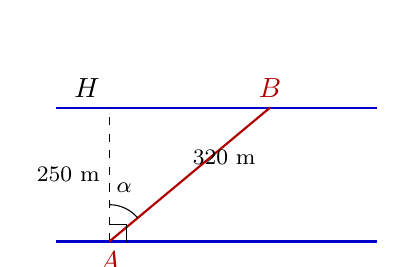
\begin{tikzpicture}[scale=0.85]
  \draw[thick, blue!80!black] (-0.8,0) -- (4,0);
  \draw[thick, blue!80!black] (-0.8,2) -- (4,2);
  \coordinate (A) at (0,0);
  \coordinate (H) at (0,2);
  \coordinate (B) at (2.4,2);
  \draw[dashed] (A) -- (H) node[above left]{$H$};
  \draw[thick, red!70!black] (A) node[below]{$A$} -- (B) node[above]{$B$};
  \draw (A) ++(0,0.25) -- ++(0.25,0) -- ++(0,-0.25);
  \draw (A) ++(0,0.55) arc (90:39.8:0.55);
  \node at (0.22,0.8) {\footnotesize $\alpha$};
  \node[left] at (0,1) {\footnotesize $250\text{ m}$};
  \node[above right] at (1.1,1) {\footnotesize $320\text{ m}$};
\end{tikzpicture}
\end{center}
\choice
{$25^\circ$}
{\True $39^\circ$}
{$45^\circ$}
{$51^\circ$}
\end{ex}

\begin{ex}
Cho đường tròn $(O; 5\text{ cm})$ và một điểm $A$ nằm ngoài đường tròn sao cho $OA = 13\text{ cm}$. Qua $A$ kẻ tiếp tuyến $AB$ với đường tròn ($B$ là tiếp điểm). Độ dài đoạn thẳng $AB$ bằng:
\choice
{\True $12\text{ cm}$}
{$8\text{ cm}$}
{$\sqrt{194}\text{ cm}$}
{$18\text{ cm}$}
\end{ex}


\vspace{1mm}
\noindent\textbf{BẢNG TRẢ LỜI TRẮC NGHIỆM PHẦN I:}
\begin{center}
\begin{tabular}{|c|c|c|c|c|c|c|c|c|c|c|c|c|}
\hline
\textbf{Câu} & \textbf{1} & \textbf{2} & \textbf{3} & \textbf{4} & \textbf{5} & \textbf{6} & \textbf{7} & \textbf{8} & \textbf{9} & \textbf{10} & \textbf{11} & \textbf{12} \\
\hline
\textbf{Chọn} & \rule{0pt}{0.65cm} & & & & & & & & & & & \\
\hline
\end{tabular}
\end{center}
\vspace{2mm}

% --- PHẦN II ---
\noindent\textbf{\large PHẦN II. CÂU TRẮC NGHIỆM ĐÚNG SAI (2,0 điểm)}

\textit{Thí sinh trả lời từ câu 1 đến câu 2. Trong mỗi ý a), b), c), d) ở mỗi câu, thí sinh chọn đúng hoặc sai.}

\vspace{1mm}
\begin{ex}
Cho hai số thực $x, y$ thỏa mãn $x > y$. Xét tính Đúng/Sai của các khẳng định sau:
\choiceTF
{\True $x - 5 > y - 5$.}
{$-4x > -4y$.}
{\True $3x - 2 > 3y - 2$.}
{\True $-2x + 1 < -2y + 1$.}
\end{ex}

\begin{ex}
Cho tam giác $DEF$ vuông tại $D$, biết $DE = 5\text{ cm}$ và $DF = 12\text{ cm}$. Xét tính Đúng/Sai của các khẳng định sau:
\choiceTF
{\True Độ dài cạnh huyền $EF = 13\text{ cm}$.}
{$\sin E = \frac{5}{13}$.}
{\True $\cos F = \frac{12}{13}$.}
{$\tan E = \frac{5}{12}$.}
\end{ex}


\vspace{1mm}
\noindent\textbf{BẢNG TRẢ LỜI ĐÚNG SAI PHẦN II:}
\begin{center}
\begin{tabular}{|c|c|c|c|c||c|c|c|c|c|}
\hline
\textbf{Câu} & \textbf{Lệnh hỏi} & \textbf{Đúng} & \textbf{Sai} & \textbf{Điểm} & \textbf{Câu} & \textbf{Lệnh hỏi} & \textbf{Đúng} & \textbf{Sai} & \textbf{Điểm} \\
\hline
 & a) & & & & & a) & & & \\
\cline{2-4}\cline{7-9}
\textbf{1} & b) & & & & \textbf{2} & b) & & & \\
\cline{2-4}\cline{7-9}
 & c) & & & & & c) & & & \\
\cline{2-4}\cline{7-9}
 & d) & & & & & d) & & & \\
\hline
\end{tabular}
\end{center}
\vspace{2mm}

% --- PHẦN III ---
\noindent\textbf{\large PHẦN III. CÂU TRẮC NGHIỆM TRẢ LỜI NGẮN (1,0 điểm)}

\textit{Thí sinh trả lời từ câu 1 đến câu 2. Viết câu trả lời vào ô quy định.}

\vspace{1mm}
\begin{ex}
Tìm $x$, biết: $\sqrt{2x - 1} = 3$.
\shortans{$x = 5$}
\end{ex}

\begin{ex}
Cho đường tròn $(O)$ có bán kính $R = 5\text{ cm}$. Khoảng cách từ tâm $O$ đến dây $AB$ bằng $3\text{ cm}$. Tính độ dài dây $AB$.
\shortans{$8\text{ cm}$}
\end{ex}


\vspace{2mm}
% --- PHẦN IV ---
\noindent\textbf{\large PHẦN IV. TỰ LUẬN (4,0 điểm)}

\textit{Thí sinh trình bày chi tiết lời giải vào giấy làm bài.}

\vspace{1mm}
\noindent\textbf{Câu 1 (2,0 điểm).}

Giải các phương trình và bất phương trình sau:\par a) $(x - 3)(x - 4) = 0$.\par b) $\frac{x + 1}{x - 1} - \frac{x + 2}{x + 2} = \frac{6}{(x - 1)(x + 2)}$.\par c) $5x + 4 < 2x - 2$.\par d) $\frac{4x + 5}{2} - \frac{5x + 6}{3} \le 1$.

\vspace{2mm}
\noindent\textbf{Câu 2 (1,0 điểm).}

Một người mua một cái bàn là và một cái quạt điện với tổng số tiền theo giá niêm yết là 750 nghìn đồng. Hiện tại cửa hàng đang thực hiện giảm giá $10\%$ đối với bàn là và $20\%$ đối với quạt điện so với giá niêm yết. Vì vậy người đó chỉ phải trả tổng cộng 625 nghìn đồng. Tính giá tiền một cái bàn là và một cái quạt điện theo giá niêm yết.

\vspace{2mm}
\noindent\textbf{Câu 3 (0,5 điểm).}

Cho tam giác $ABC$ vuông tại $A$ có $\widehat{C} = 30^\circ$, cạnh $AB = 8\text{ cm}$. Tính:\par a) Số đo góc $B$.\par b) Độ dài các cạnh $AC$ và $BC$.

\vspace{2mm}
\noindent\textbf{Câu 4 (0,5 điểm).}

Cho tam giác $ABC$ vuông tại $A$, đường cao $AH$. Chứng minh rằng $AH \cdot BC = AB \cdot AC$.

\vspace{2mm}

\vfill
\begin{center}
  \textbf{--- HẾT ---}
\end{center}
\end{document}
